\chapter{Enemies and their Discontents} 

\lstset{style=6502Style}

\begin{q}{Jeff Minter's Development Diary in Zzap Magazine\cite{planner}}
ACONT 

This is the bit that I knew would take me ages to write and get glitch
free, and the bit that is absolutely necessary to the functioning of the game.
The module ACONT is essentially an interpreter for my own 'wave language',
allowing me to describe, exactly, an attack wave in about 50 bytes of data. The
waves for the first part of IRIDIS are in good rollicking shoot-'em-up style,
and there have to be plenty of them. There are five planets and each planet is
to have twenty levels associated with it. It's impractical to write separate
bits of code for each wave; even with 64K you can run outta memory pretty fast
that way, and it's not really necessary coz a lot of stuff would be duplicated.
Hence ACONT.

\end{q}

The bits and bytes that define the behaviour and appearance of
wave after wave of Iridis Alpha's enemy formations - twenty across each of the
five planets giving on hundred in all - takes up relatively little space given
the sheer variety of adversaries the player faces.

\subsection{You're a Waste of Space}
Each 'wave' of enemies is defined by a 40 byte data structure, not 50 bytes as
Minter initially suggested in his development diary. There's a little bit of 
waste going on in here too, bytes 10 to 14 are unused, while \icode{Byte 15} is only
ever set (to \icode{\$01}) by the wave data structure that describes the default explosion 
behaviour for enemy ships.

As we can see here, the sole purpose of \icode{Byte 15} is to determine whether a
new set of wave data needs to be loaded. This makes sense, once the animation is finished
we'll need to load a new enemy ship. Still, you can't help thinking there might have been 
a way that didn't waste 99 bytes! 

\CopyPartialFile{../iridisalpha/src/iridisalpha.asm}{tmp.asm}{1962}{1981}%
\lstinputlisting[caption="Routine for Animating Enemy Sprites",basicstyle=\tiny]{tmp.asm}

And actually, it's more than that because as we shall see the \icode{ACONT} 40-byte data
structure is defined more than once per wave. Separate instances are defined for later
phases of the enemy ship, such as when it is first hit. Early examples of this in the game
are the 'spinning rings' you get when you hit an enemy in the first level.

In all there are 200 instances of the \icode{ACONT} data structure: 100 defining each of the
enemy waves and another 100 defining the subsequent behaviour of the ships when hit. There isn't
a one-to-one mapping here either - many of the effects are reused across levels and as we shall
see there can be multiple stages in an enemy's lifecycle.

So there's already 1000 bytes or 1 kilobyte of wasted space in the level data due to bytes
that are never or rarely used. That's out of a total of 8 kilobytes actually used.

Shocking stuff. Awful.

\subsection{And You're a Waste of Space}

\icode{Bytes 33 - 34} seem to be left in an unfinished state. Wave 12 on Planet 5 has both populated, \icode{flowchartArrowAsExplosion}
is the only other wave that has anything in either byte, in this case \icode{\$60} in \icode{Byte 33}.

This another 200 wasted bytes it seems but it seems these bytes have some game logic attached and
when you look at what that logic is doing it seems broken.

\CopyPartialFile{../iridisalpha/src/iridisalpha.asm}{tmp.asm}{1945}{1958}%
\lstinputlisting[caption="Routine for Animating Enemy Sprites",basicstyle=\tiny]{tmp.asm}

When Byte 34 (\icode{\$21}) is populated (and fire has not been pressed) the game will attempt to load
a set of wave date from Bytes 33 and 34:

\CopyPartialFile{../iridisalpha/src/iridisalpha.asm}{tmp.asm}{1974}{1992}%
\lstinputlisting[caption="Routine for Animating Enemy Sprites",basicstyle=\tiny]{tmp.asm}

In the case of the data for Planet 5 Level 12 this translates to whatever is at \icode{\$1488}. As it happens this 
is the address of the frequency data used in the title screen's music. So effectively pretty random data:

\CopyPartialFile{../iridisalpha/src/iridisalpha.asm}{tmp.asm}{659}{674}%
\lstinputlisting[caption="Routine for Animating Enemy Sprites",basicstyle=\tiny]{tmp.asm}

Clearly, no one has ever reached level 12 in planet 5!

\subsection{Clever Business}
\begin{q}{Jeff Minter's Development Diary in Zzap Magazine\cite{planner}}
You pass the interpreter data, that describes exactly stuff like: what each
alien looks like, how many frames of animation it uses, speed of that
animation, colour, velocities in X— and Y— directions, accelerations in X and
Y, whether the alien should 'home in' on a target, and if so, what to home in
on; whether an alien is subject to gravity, and if so, how strong is the
gravity; what the alien should do if it hits top of screen, the ground, one of
your bullets, or you; whether the alien can fire bullets, and if so, how
frequently, and what types; how many points you get if you shoot it, and how
much damage it does if it hits you; and a whole bunch more stuff like that. As
you can imagine it was a fairly heavy routine to write and get debugged, but
that's done now; took me about three weeks in all I'd say.
\end{q}

The level data does actually define some of this stuff. It does so by making
heavy use of a simple but clever trick that in its way is very specific to
8-bit assembly programming: storing references to other data structures as
a pair of bytes. We've discussed the way this works previously but we'll try
again briefly here as it won't do any harm. 

The 40-byte data structure that defines the default explosion animation (and
behaviour, so far as it goes) is stored at position \icode{\$18C8} while the
game is running. To use this explosion data when an enemy is killed, bytes 31
and 32 of the data structure contain the values \icode{\$C8,\$18}. 

When an enemy is hit, the game routine responsible for figuring out what to do next
with it looks at bytes 31 and 32 and loads in the data structure at the address
given by combining \icode{\$18} and \icode{\$C8} as the 'new' wave data that
defines how that enemy ship will now behave. Since the data structure at
\icode{\$18C8} basically says: animate an explosion sprite and don't move
anywhere that is exactly what the enemy ship now does.

Here's the explosion data structure, which we've labelled \icode{defaultExplosion} in
our disassembly, in the first twenty bytes or so of it's gory detail:

\CopyPartialFile{../iridisalpha/src/level_data/level_data2.asm}{tmp.asm}{4276}{4311}%
\lstinputlisting[caption="Routine for Animating Enemy Sprites",basicstyle=\tiny]{tmp.asm}

We can see the first 7 bytes are concerned with the appearance and basic behaviour of the
enemy. Bytes 2 and 3 define the sprite used for display on the upper planet, Bytes 5 and 6
for the lower planet. The reason there's two in each case is because they are describing the
start and end point of the sprite's animation. The game will display \icode{EXPLOSION\_START} \icode{\$ED}) first,
then cycle through the next two sprites until it reaches \icode{EXPLOSION\_START} + 3 (\icode{\$F0}). 

\subsection{Sprites Behaving Badly}

We can see this in action in \icode{AnimateAttackShipSprites}. When this routine runs Byte 4 has been loaded
to \icode{upperPlanetAttackShipInitialFrameRate} for the upper planet and \icode{lowerPlanetAttackShipInitialFrameRate}
for the lower planet. This routine is cycling through the sprites given by Byte 2 as the lower limit and Byte 3 as 
the upper limit. This is what the animation consists of: an animation effect achieved by changing the sprite from
one to another to create a classic animation effect.

\CopyPartialFile{../iridisalpha/src/iridisalpha.asm}{tmp.asm}{8223}{8258}%
\lstinputlisting[caption="Routine for Animating Enemy Sprites",basicstyle=\tiny]{tmp.asm}
 
Byte 2 (loaded to \icode{upperPlanetAttackShipAnimationFrameRate} comes into play here. It's decremented and as long as it's
not zero yet the animation is skipped, execution jumps forward to \icode{AnimateLowerPlanetAttackShips}:

\CopyPartialFile{../iridisalpha/src/iridisalpha.asm}{tmp.asm}{8235}{8237}%
\lstinputlisting[caption="Routine for Animating Enemy Sprites",basicstyle=\tiny]{tmp.asm}

If it is zero, it instead gets reset to the initial value from Byte 2 (stored in
 \icode{upperPlanetAttackShipInitialFrameRate})
and the current sprite for the enemy ship is incremented to point to the next 'frame' of the ship's animation:

\CopyPartialFile{../iridisalpha/src/iridisalpha.asm}{tmp.asm}{8239}{8242}%
\lstinputlisting[caption="Routine for Animating Enemy Sprites",basicstyle=\tiny]{tmp.asm}

Next we check if we've reached the end of the animation by checking the value
of Byte 3 (loaded to \icode{upperPlanetAttackShipSpriteAnimationEnd}).  If so,
we reset \icode{upperPlanetAttackShip2SpriteValue} to the value initially
loaded from Byte 2 - and that is what will be used to display the ship the next
time we pass through to animate the ship:

\CopyPartialFile{../iridisalpha/src/iridisalpha.asm}{tmp.asm}{8244}{8251}%
\lstinputlisting[caption="Routine for Animating Enemy Sprites",basicstyle=\tiny]{tmp.asm}

\begin{figure}[H]
  {
    \setlength{\tabcolsep}{3.0pt}
    \setlength\cmidrulewidth{\heavyrulewidth} % Make cmidrule = 
	\centering
	\begin{subfigure}{0.3\textwidth}
		
\begin{figure}[H]
  {
    \setlength{\tabcolsep}{3.0pt}
    \setlength\cmidrulewidth{\heavyrulewidth} % Make cmidrule = 
    \begin{adjustbox}{width=3cm,center}
      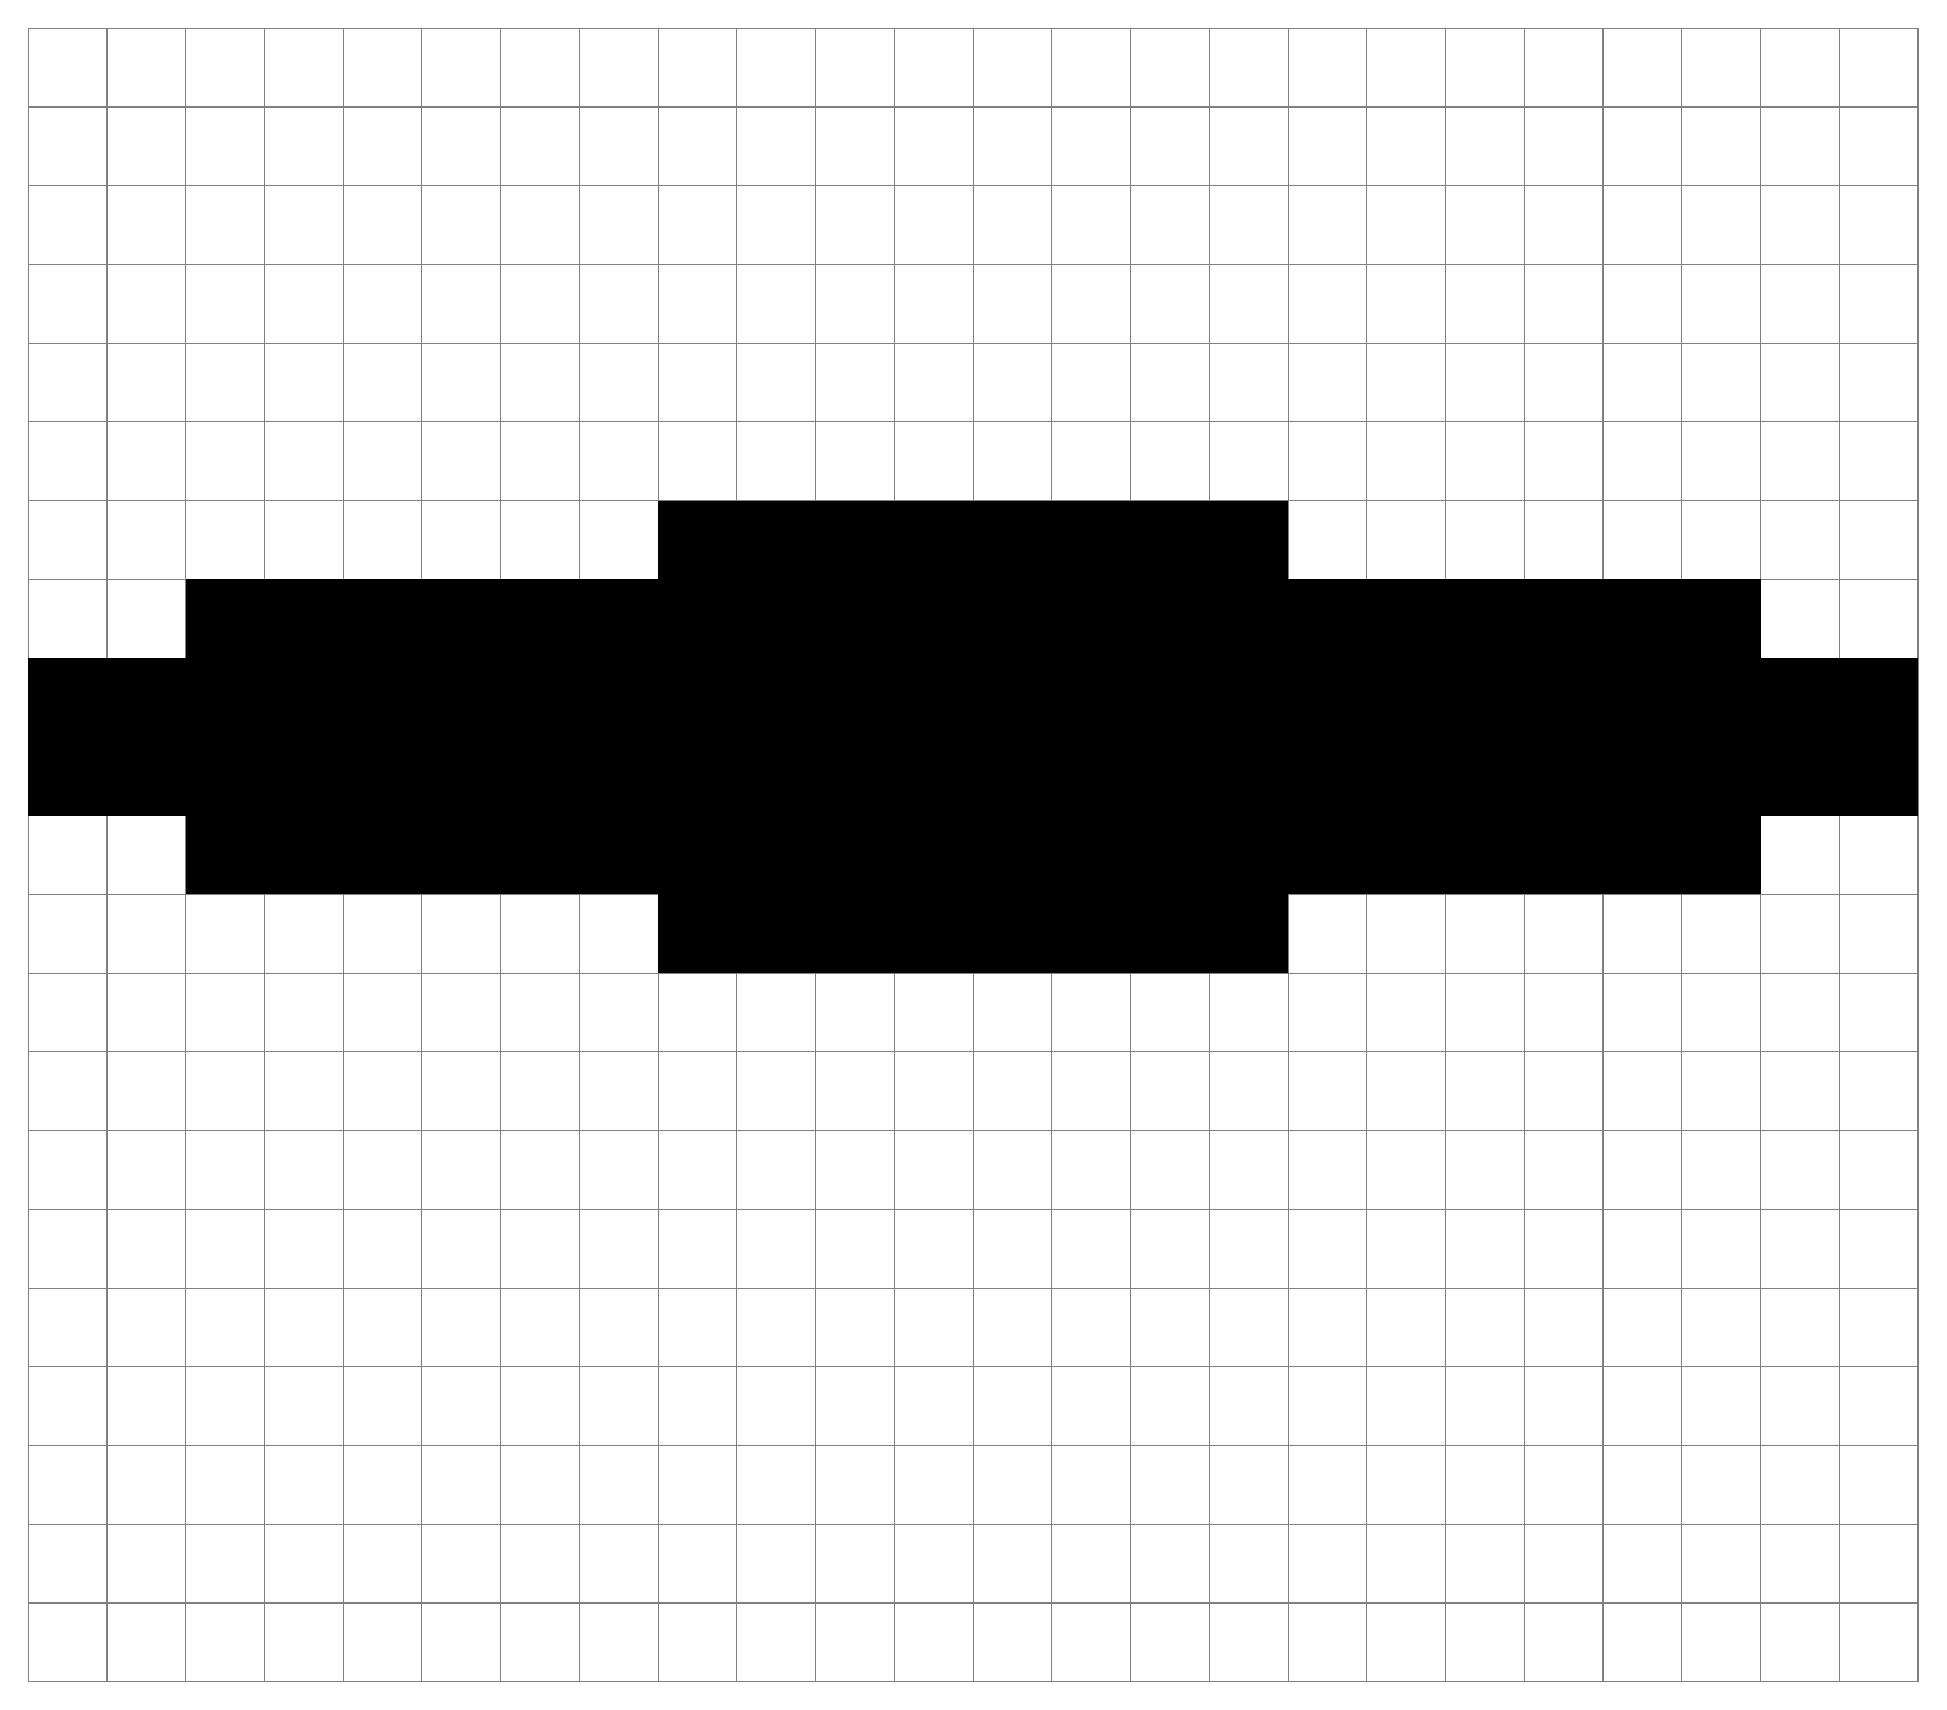
\begin{tikzpicture}

	\draw[step=1.0,gray,thin] (0,0) grid (24,21);
	\fill[\SPRITECOLOR] (8,14) rectangle ++ (1,1);
	\fill[\SPRITECOLOR] (9,14) rectangle ++ (1,1);
	\fill[\SPRITECOLOR] (10,14) rectangle ++ (1,1);
	\fill[\SPRITECOLOR] (11,14) rectangle ++ (1,1);
	\fill[\SPRITECOLOR] (12,14) rectangle ++ (1,1);
	\fill[\SPRITECOLOR] (13,14) rectangle ++ (1,1);
	\fill[\SPRITECOLOR] (14,14) rectangle ++ (1,1);
	\fill[\SPRITECOLOR] (15,14) rectangle ++ (1,1);
	\fill[\SPRITECOLOR] (2,13) rectangle ++ (1,1);
	\fill[\SPRITECOLOR] (3,13) rectangle ++ (1,1);
	\fill[\SPRITECOLOR] (4,13) rectangle ++ (1,1);
	\fill[\SPRITECOLOR] (5,13) rectangle ++ (1,1);
	\fill[\SPRITECOLOR] (6,13) rectangle ++ (1,1);
	\fill[\SPRITECOLOR] (7,13) rectangle ++ (1,1);
	\fill[\SPRITECOLOR] (8,13) rectangle ++ (1,1);
	\fill[\SPRITECOLOR] (9,13) rectangle ++ (1,1);
	\fill[\SPRITECOLOR] (10,13) rectangle ++ (1,1);
	\fill[\SPRITECOLOR] (11,13) rectangle ++ (1,1);
	\fill[\SPRITECOLOR] (12,13) rectangle ++ (1,1);
	\fill[\SPRITECOLOR] (13,13) rectangle ++ (1,1);
	\fill[\SPRITECOLOR] (14,13) rectangle ++ (1,1);
	\fill[\SPRITECOLOR] (15,13) rectangle ++ (1,1);
	\fill[\SPRITECOLOR] (16,13) rectangle ++ (1,1);
	\fill[\SPRITECOLOR] (17,13) rectangle ++ (1,1);
	\fill[\SPRITECOLOR] (18,13) rectangle ++ (1,1);
	\fill[\SPRITECOLOR] (19,13) rectangle ++ (1,1);
	\fill[\SPRITECOLOR] (20,13) rectangle ++ (1,1);
	\fill[\SPRITECOLOR] (21,13) rectangle ++ (1,1);
	\fill[\MULTICOLORTWO] (0,12) rectangle ++ (1,1);
	\fill[\MULTICOLORTWO] (1,12) rectangle ++ (1,1);
	\fill[\MULTICOLORTWO] (2,12) rectangle ++ (1,1);
	\fill[\MULTICOLORTWO] (3,12) rectangle ++ (1,1);
	\fill[\MULTICOLORTWO] (4,12) rectangle ++ (1,1);
	\fill[\MULTICOLORTWO] (5,12) rectangle ++ (1,1);
	\fill[\MULTICOLORONE] (6,12) rectangle ++ (1,1);
	\fill[\MULTICOLORONE] (7,12) rectangle ++ (1,1);
	\fill[\MULTICOLORONE] (8,12) rectangle ++ (1,1);
	\fill[\MULTICOLORONE] (9,12) rectangle ++ (1,1);
	\fill[\MULTICOLORONE] (10,12) rectangle ++ (1,1);
	\fill[\MULTICOLORONE] (11,12) rectangle ++ (1,1);
	\fill[\MULTICOLORTWO] (12,12) rectangle ++ (1,1);
	\fill[\MULTICOLORTWO] (13,12) rectangle ++ (1,1);
	\fill[\MULTICOLORTWO] (14,12) rectangle ++ (1,1);
	\fill[\MULTICOLORTWO] (15,12) rectangle ++ (1,1);
	\fill[\MULTICOLORTWO] (16,12) rectangle ++ (1,1);
	\fill[\MULTICOLORTWO] (17,12) rectangle ++ (1,1);
	\fill[\MULTICOLORONE] (18,12) rectangle ++ (1,1);
	\fill[\MULTICOLORONE] (19,12) rectangle ++ (1,1);
	\fill[\MULTICOLORONE] (20,12) rectangle ++ (1,1);
	\fill[\MULTICOLORONE] (21,12) rectangle ++ (1,1);
	\fill[\MULTICOLORONE] (22,12) rectangle ++ (1,1);
	\fill[\MULTICOLORONE] (23,12) rectangle ++ (1,1);
	\fill[\MULTICOLORTWO] (0,11) rectangle ++ (1,1);
	\fill[\MULTICOLORTWO] (1,11) rectangle ++ (1,1);
	\fill[\MULTICOLORTWO] (2,11) rectangle ++ (1,1);
	\fill[\MULTICOLORTWO] (3,11) rectangle ++ (1,1);
	\fill[\MULTICOLORTWO] (4,11) rectangle ++ (1,1);
	\fill[\MULTICOLORTWO] (5,11) rectangle ++ (1,1);
	\fill[\MULTICOLORONE] (6,11) rectangle ++ (1,1);
	\fill[\MULTICOLORONE] (7,11) rectangle ++ (1,1);
	\fill[\MULTICOLORONE] (8,11) rectangle ++ (1,1);
	\fill[\MULTICOLORONE] (9,11) rectangle ++ (1,1);
	\fill[\MULTICOLORONE] (10,11) rectangle ++ (1,1);
	\fill[\MULTICOLORONE] (11,11) rectangle ++ (1,1);
	\fill[\MULTICOLORTWO] (12,11) rectangle ++ (1,1);
	\fill[\MULTICOLORTWO] (13,11) rectangle ++ (1,1);
	\fill[\MULTICOLORTWO] (14,11) rectangle ++ (1,1);
	\fill[\MULTICOLORTWO] (15,11) rectangle ++ (1,1);
	\fill[\MULTICOLORTWO] (16,11) rectangle ++ (1,1);
	\fill[\MULTICOLORTWO] (17,11) rectangle ++ (1,1);
	\fill[\MULTICOLORONE] (18,11) rectangle ++ (1,1);
	\fill[\MULTICOLORONE] (19,11) rectangle ++ (1,1);
	\fill[\MULTICOLORONE] (20,11) rectangle ++ (1,1);
	\fill[\MULTICOLORONE] (21,11) rectangle ++ (1,1);
	\fill[\MULTICOLORONE] (22,11) rectangle ++ (1,1);
	\fill[\MULTICOLORONE] (23,11) rectangle ++ (1,1);
	\fill[\SPRITECOLOR] (2,10) rectangle ++ (1,1);
	\fill[\SPRITECOLOR] (3,10) rectangle ++ (1,1);
	\fill[\SPRITECOLOR] (4,10) rectangle ++ (1,1);
	\fill[\SPRITECOLOR] (5,10) rectangle ++ (1,1);
	\fill[\SPRITECOLOR] (6,10) rectangle ++ (1,1);
	\fill[\SPRITECOLOR] (7,10) rectangle ++ (1,1);
	\fill[\SPRITECOLOR] (8,10) rectangle ++ (1,1);
	\fill[\SPRITECOLOR] (9,10) rectangle ++ (1,1);
	\fill[\SPRITECOLOR] (10,10) rectangle ++ (1,1);
	\fill[\SPRITECOLOR] (11,10) rectangle ++ (1,1);
	\fill[\SPRITECOLOR] (12,10) rectangle ++ (1,1);
	\fill[\SPRITECOLOR] (13,10) rectangle ++ (1,1);
	\fill[\SPRITECOLOR] (14,10) rectangle ++ (1,1);
	\fill[\SPRITECOLOR] (15,10) rectangle ++ (1,1);
	\fill[\SPRITECOLOR] (16,10) rectangle ++ (1,1);
	\fill[\SPRITECOLOR] (17,10) rectangle ++ (1,1);
	\fill[\SPRITECOLOR] (18,10) rectangle ++ (1,1);
	\fill[\SPRITECOLOR] (19,10) rectangle ++ (1,1);
	\fill[\SPRITECOLOR] (20,10) rectangle ++ (1,1);
	\fill[\SPRITECOLOR] (21,10) rectangle ++ (1,1);
	\fill[\SPRITECOLOR] (8,9) rectangle ++ (1,1);
	\fill[\SPRITECOLOR] (9,9) rectangle ++ (1,1);
	\fill[\SPRITECOLOR] (10,9) rectangle ++ (1,1);
	\fill[\SPRITECOLOR] (11,9) rectangle ++ (1,1);
	\fill[\SPRITECOLOR] (12,9) rectangle ++ (1,1);
	\fill[\SPRITECOLOR] (13,9) rectangle ++ (1,1);
	\fill[\SPRITECOLOR] (14,9) rectangle ++ (1,1);
	\fill[\SPRITECOLOR] (15,9) rectangle ++ (1,1);

      \end{tikzpicture}
    \end{adjustbox}
  }\caption{FLYING\_SAUCER1}
\end{figure}

	\end{subfigure}
	\begin{subfigure}{0.3\textwidth}
		
\begin{figure}[H]
  {
    \setlength{\tabcolsep}{3.0pt}
    \setlength\cmidrulewidth{\heavyrulewidth} % Make cmidrule = 
    \begin{adjustbox}{width=3cm,center}
      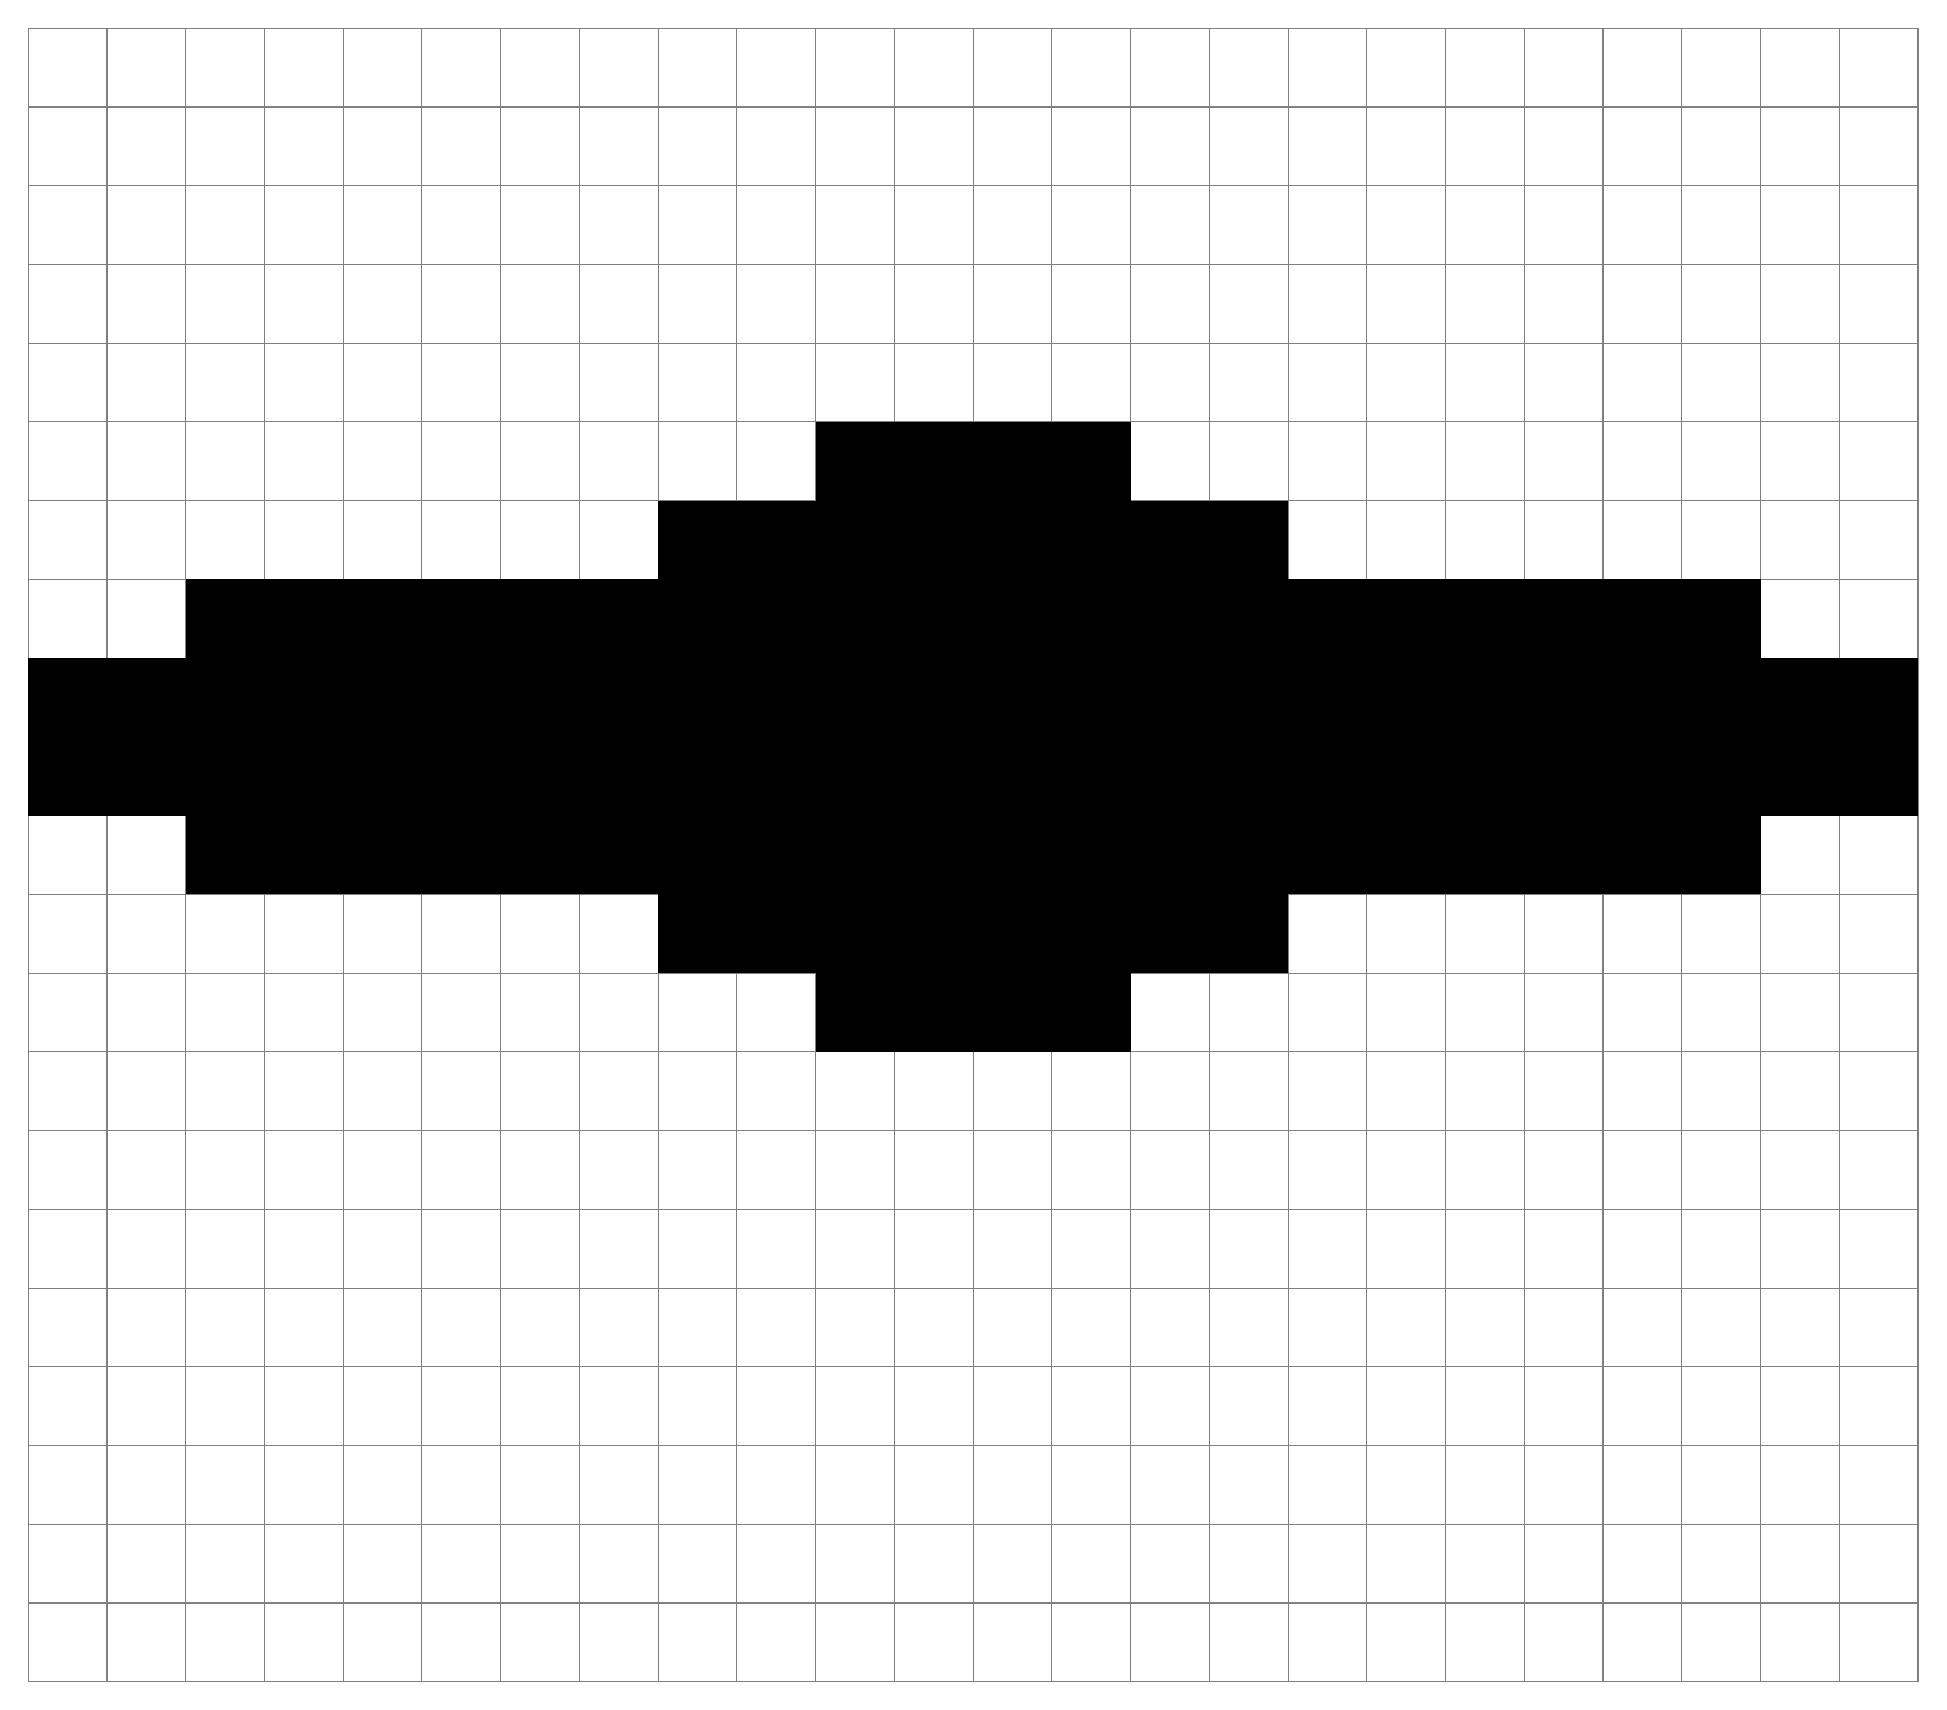
\begin{tikzpicture}

	\draw[step=1.0,gray,thin] (0,0) grid (24,21);
	\fill[\MULTICOLORONE] (10,15) rectangle ++ (1,1);
	\fill[\MULTICOLORONE] (11,15) rectangle ++ (1,1);
	\fill[\MULTICOLORONE] (12,15) rectangle ++ (1,1);
	\fill[\MULTICOLORONE] (13,15) rectangle ++ (1,1);
	\fill[\SPRITECOLOR] (8,14) rectangle ++ (1,1);
	\fill[\SPRITECOLOR] (9,14) rectangle ++ (1,1);
	\fill[\SPRITECOLOR] (10,14) rectangle ++ (1,1);
	\fill[\SPRITECOLOR] (11,14) rectangle ++ (1,1);
	\fill[\SPRITECOLOR] (12,14) rectangle ++ (1,1);
	\fill[\SPRITECOLOR] (13,14) rectangle ++ (1,1);
	\fill[\SPRITECOLOR] (14,14) rectangle ++ (1,1);
	\fill[\SPRITECOLOR] (15,14) rectangle ++ (1,1);
	\fill[\SPRITECOLOR] (2,13) rectangle ++ (1,1);
	\fill[\SPRITECOLOR] (3,13) rectangle ++ (1,1);
	\fill[\SPRITECOLOR] (4,13) rectangle ++ (1,1);
	\fill[\SPRITECOLOR] (5,13) rectangle ++ (1,1);
	\fill[\SPRITECOLOR] (6,13) rectangle ++ (1,1);
	\fill[\SPRITECOLOR] (7,13) rectangle ++ (1,1);
	\fill[\SPRITECOLOR] (8,13) rectangle ++ (1,1);
	\fill[\SPRITECOLOR] (9,13) rectangle ++ (1,1);
	\fill[\SPRITECOLOR] (10,13) rectangle ++ (1,1);
	\fill[\SPRITECOLOR] (11,13) rectangle ++ (1,1);
	\fill[\SPRITECOLOR] (12,13) rectangle ++ (1,1);
	\fill[\SPRITECOLOR] (13,13) rectangle ++ (1,1);
	\fill[\SPRITECOLOR] (14,13) rectangle ++ (1,1);
	\fill[\SPRITECOLOR] (15,13) rectangle ++ (1,1);
	\fill[\SPRITECOLOR] (16,13) rectangle ++ (1,1);
	\fill[\SPRITECOLOR] (17,13) rectangle ++ (1,1);
	\fill[\SPRITECOLOR] (18,13) rectangle ++ (1,1);
	\fill[\SPRITECOLOR] (19,13) rectangle ++ (1,1);
	\fill[\SPRITECOLOR] (20,13) rectangle ++ (1,1);
	\fill[\SPRITECOLOR] (21,13) rectangle ++ (1,1);
	\fill[\MULTICOLORTWO] (0,12) rectangle ++ (1,1);
	\fill[\MULTICOLORTWO] (1,12) rectangle ++ (1,1);
	\fill[\MULTICOLORONE] (2,12) rectangle ++ (1,1);
	\fill[\MULTICOLORONE] (3,12) rectangle ++ (1,1);
	\fill[\MULTICOLORONE] (4,12) rectangle ++ (1,1);
	\fill[\MULTICOLORONE] (5,12) rectangle ++ (1,1);
	\fill[\MULTICOLORONE] (6,12) rectangle ++ (1,1);
	\fill[\MULTICOLORONE] (7,12) rectangle ++ (1,1);
	\fill[\MULTICOLORTWO] (8,12) rectangle ++ (1,1);
	\fill[\MULTICOLORTWO] (9,12) rectangle ++ (1,1);
	\fill[\MULTICOLORTWO] (10,12) rectangle ++ (1,1);
	\fill[\MULTICOLORTWO] (11,12) rectangle ++ (1,1);
	\fill[\MULTICOLORTWO] (12,12) rectangle ++ (1,1);
	\fill[\MULTICOLORTWO] (13,12) rectangle ++ (1,1);
	\fill[\MULTICOLORONE] (14,12) rectangle ++ (1,1);
	\fill[\MULTICOLORONE] (15,12) rectangle ++ (1,1);
	\fill[\MULTICOLORONE] (16,12) rectangle ++ (1,1);
	\fill[\MULTICOLORONE] (17,12) rectangle ++ (1,1);
	\fill[\MULTICOLORONE] (18,12) rectangle ++ (1,1);
	\fill[\MULTICOLORONE] (19,12) rectangle ++ (1,1);
	\fill[\MULTICOLORTWO] (20,12) rectangle ++ (1,1);
	\fill[\MULTICOLORTWO] (21,12) rectangle ++ (1,1);
	\fill[\MULTICOLORTWO] (22,12) rectangle ++ (1,1);
	\fill[\MULTICOLORTWO] (23,12) rectangle ++ (1,1);
	\fill[\MULTICOLORTWO] (0,11) rectangle ++ (1,1);
	\fill[\MULTICOLORTWO] (1,11) rectangle ++ (1,1);
	\fill[\MULTICOLORONE] (2,11) rectangle ++ (1,1);
	\fill[\MULTICOLORONE] (3,11) rectangle ++ (1,1);
	\fill[\MULTICOLORONE] (4,11) rectangle ++ (1,1);
	\fill[\MULTICOLORONE] (5,11) rectangle ++ (1,1);
	\fill[\MULTICOLORONE] (6,11) rectangle ++ (1,1);
	\fill[\MULTICOLORONE] (7,11) rectangle ++ (1,1);
	\fill[\MULTICOLORTWO] (8,11) rectangle ++ (1,1);
	\fill[\MULTICOLORTWO] (9,11) rectangle ++ (1,1);
	\fill[\MULTICOLORTWO] (10,11) rectangle ++ (1,1);
	\fill[\MULTICOLORTWO] (11,11) rectangle ++ (1,1);
	\fill[\MULTICOLORTWO] (12,11) rectangle ++ (1,1);
	\fill[\MULTICOLORTWO] (13,11) rectangle ++ (1,1);
	\fill[\MULTICOLORONE] (14,11) rectangle ++ (1,1);
	\fill[\MULTICOLORONE] (15,11) rectangle ++ (1,1);
	\fill[\MULTICOLORONE] (16,11) rectangle ++ (1,1);
	\fill[\MULTICOLORONE] (17,11) rectangle ++ (1,1);
	\fill[\MULTICOLORONE] (18,11) rectangle ++ (1,1);
	\fill[\MULTICOLORONE] (19,11) rectangle ++ (1,1);
	\fill[\MULTICOLORTWO] (20,11) rectangle ++ (1,1);
	\fill[\MULTICOLORTWO] (21,11) rectangle ++ (1,1);
	\fill[\MULTICOLORTWO] (22,11) rectangle ++ (1,1);
	\fill[\MULTICOLORTWO] (23,11) rectangle ++ (1,1);
	\fill[\SPRITECOLOR] (2,10) rectangle ++ (1,1);
	\fill[\SPRITECOLOR] (3,10) rectangle ++ (1,1);
	\fill[\SPRITECOLOR] (4,10) rectangle ++ (1,1);
	\fill[\SPRITECOLOR] (5,10) rectangle ++ (1,1);
	\fill[\SPRITECOLOR] (6,10) rectangle ++ (1,1);
	\fill[\SPRITECOLOR] (7,10) rectangle ++ (1,1);
	\fill[\SPRITECOLOR] (8,10) rectangle ++ (1,1);
	\fill[\SPRITECOLOR] (9,10) rectangle ++ (1,1);
	\fill[\SPRITECOLOR] (10,10) rectangle ++ (1,1);
	\fill[\SPRITECOLOR] (11,10) rectangle ++ (1,1);
	\fill[\SPRITECOLOR] (12,10) rectangle ++ (1,1);
	\fill[\SPRITECOLOR] (13,10) rectangle ++ (1,1);
	\fill[\SPRITECOLOR] (14,10) rectangle ++ (1,1);
	\fill[\SPRITECOLOR] (15,10) rectangle ++ (1,1);
	\fill[\SPRITECOLOR] (16,10) rectangle ++ (1,1);
	\fill[\SPRITECOLOR] (17,10) rectangle ++ (1,1);
	\fill[\SPRITECOLOR] (18,10) rectangle ++ (1,1);
	\fill[\SPRITECOLOR] (19,10) rectangle ++ (1,1);
	\fill[\SPRITECOLOR] (20,10) rectangle ++ (1,1);
	\fill[\SPRITECOLOR] (21,10) rectangle ++ (1,1);
	\fill[\SPRITECOLOR] (8,9) rectangle ++ (1,1);
	\fill[\SPRITECOLOR] (9,9) rectangle ++ (1,1);
	\fill[\SPRITECOLOR] (10,9) rectangle ++ (1,1);
	\fill[\SPRITECOLOR] (11,9) rectangle ++ (1,1);
	\fill[\SPRITECOLOR] (12,9) rectangle ++ (1,1);
	\fill[\SPRITECOLOR] (13,9) rectangle ++ (1,1);
	\fill[\SPRITECOLOR] (14,9) rectangle ++ (1,1);
	\fill[\SPRITECOLOR] (15,9) rectangle ++ (1,1);
	\fill[\MULTICOLORONE] (10,8) rectangle ++ (1,1);
	\fill[\MULTICOLORONE] (11,8) rectangle ++ (1,1);
	\fill[\MULTICOLORONE] (12,8) rectangle ++ (1,1);
	\fill[\MULTICOLORONE] (13,8) rectangle ++ (1,1);

      \end{tikzpicture}
    \end{adjustbox}
  }\caption{FLYING\_SAUCER2}
\end{figure}

	\end{subfigure}
	\begin{subfigure}{0.3\textwidth}
		
\begin{figure}[H]
  {
    \setlength{\tabcolsep}{3.0pt}
    \setlength\cmidrulewidth{\heavyrulewidth} % Make cmidrule = 
    \begin{adjustbox}{width=3cm,center}
      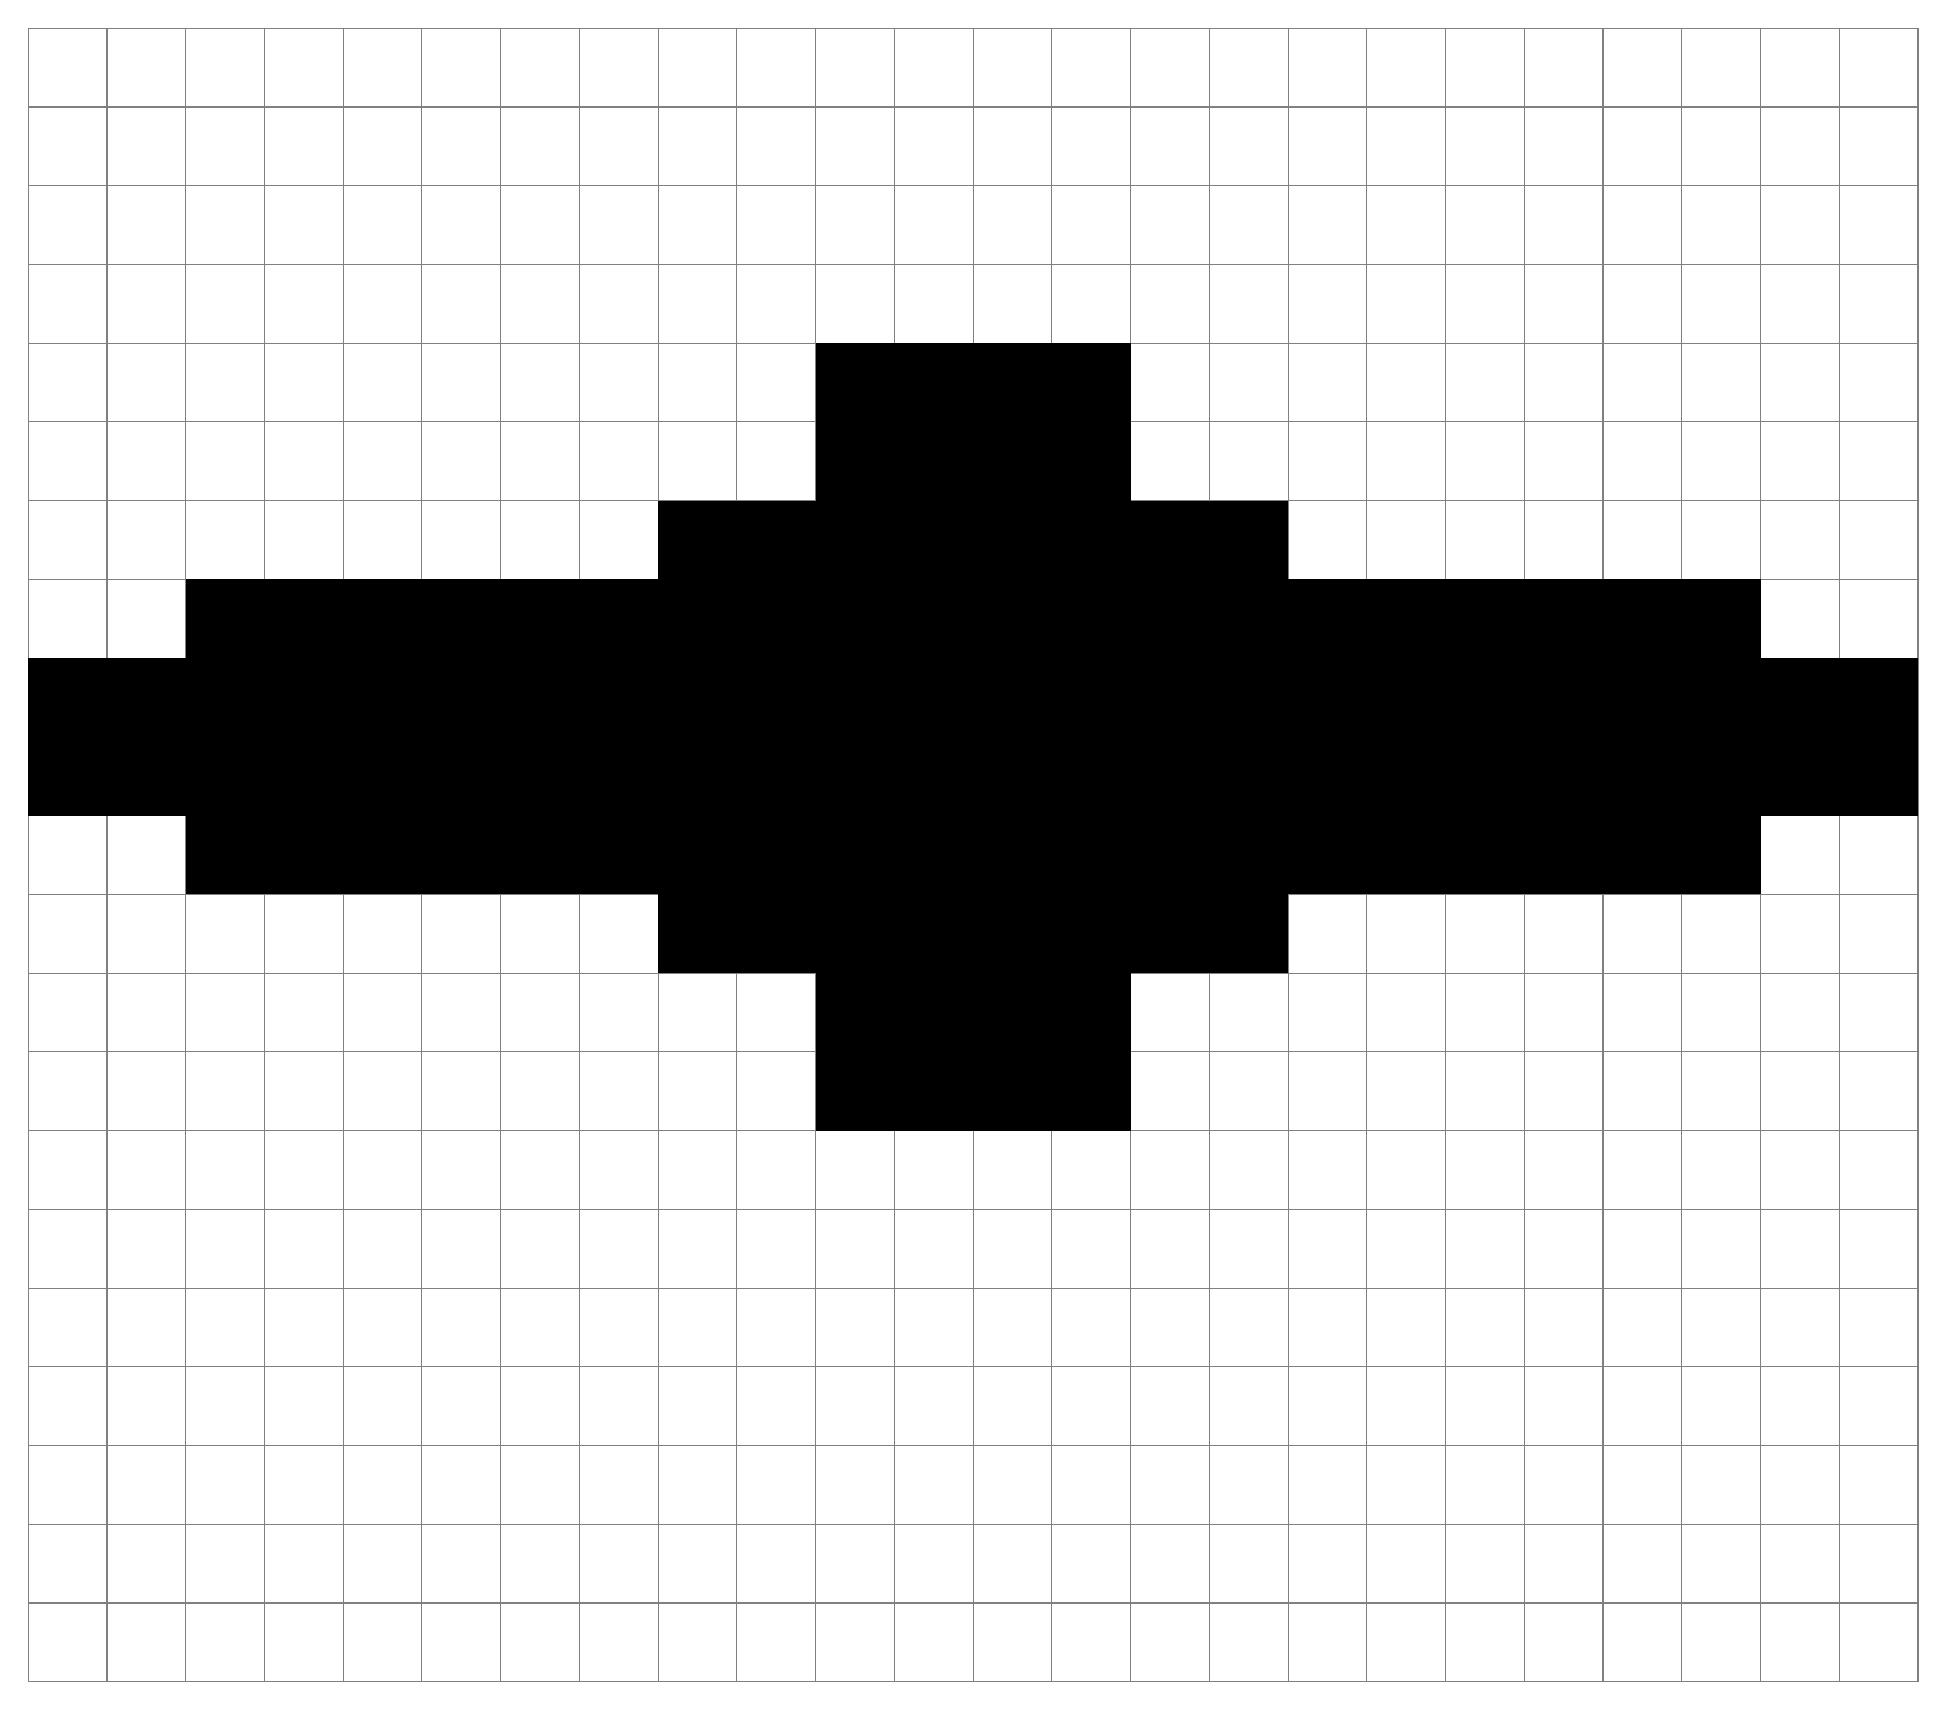
\begin{tikzpicture}

	\draw[step=1.0,gray,thin] (0,0) grid (24,21);
	\fill[\MULTICOLORTWO] (10,16) rectangle ++ (1,1);
	\fill[\MULTICOLORTWO] (11,16) rectangle ++ (1,1);
	\fill[\MULTICOLORTWO] (12,16) rectangle ++ (1,1);
	\fill[\MULTICOLORTWO] (13,16) rectangle ++ (1,1);
	\fill[\MULTICOLORONE] (10,15) rectangle ++ (1,1);
	\fill[\MULTICOLORONE] (11,15) rectangle ++ (1,1);
	\fill[\MULTICOLORONE] (12,15) rectangle ++ (1,1);
	\fill[\MULTICOLORONE] (13,15) rectangle ++ (1,1);
	\fill[\SPRITECOLOR] (8,14) rectangle ++ (1,1);
	\fill[\SPRITECOLOR] (9,14) rectangle ++ (1,1);
	\fill[\SPRITECOLOR] (10,14) rectangle ++ (1,1);
	\fill[\SPRITECOLOR] (11,14) rectangle ++ (1,1);
	\fill[\SPRITECOLOR] (12,14) rectangle ++ (1,1);
	\fill[\SPRITECOLOR] (13,14) rectangle ++ (1,1);
	\fill[\SPRITECOLOR] (14,14) rectangle ++ (1,1);
	\fill[\SPRITECOLOR] (15,14) rectangle ++ (1,1);
	\fill[\SPRITECOLOR] (2,13) rectangle ++ (1,1);
	\fill[\SPRITECOLOR] (3,13) rectangle ++ (1,1);
	\fill[\SPRITECOLOR] (4,13) rectangle ++ (1,1);
	\fill[\SPRITECOLOR] (5,13) rectangle ++ (1,1);
	\fill[\SPRITECOLOR] (6,13) rectangle ++ (1,1);
	\fill[\SPRITECOLOR] (7,13) rectangle ++ (1,1);
	\fill[\SPRITECOLOR] (8,13) rectangle ++ (1,1);
	\fill[\SPRITECOLOR] (9,13) rectangle ++ (1,1);
	\fill[\SPRITECOLOR] (10,13) rectangle ++ (1,1);
	\fill[\SPRITECOLOR] (11,13) rectangle ++ (1,1);
	\fill[\SPRITECOLOR] (12,13) rectangle ++ (1,1);
	\fill[\SPRITECOLOR] (13,13) rectangle ++ (1,1);
	\fill[\SPRITECOLOR] (14,13) rectangle ++ (1,1);
	\fill[\SPRITECOLOR] (15,13) rectangle ++ (1,1);
	\fill[\SPRITECOLOR] (16,13) rectangle ++ (1,1);
	\fill[\SPRITECOLOR] (17,13) rectangle ++ (1,1);
	\fill[\SPRITECOLOR] (18,13) rectangle ++ (1,1);
	\fill[\SPRITECOLOR] (19,13) rectangle ++ (1,1);
	\fill[\SPRITECOLOR] (20,13) rectangle ++ (1,1);
	\fill[\SPRITECOLOR] (21,13) rectangle ++ (1,1);
	\fill[\MULTICOLORONE] (0,12) rectangle ++ (1,1);
	\fill[\MULTICOLORONE] (1,12) rectangle ++ (1,1);
	\fill[\MULTICOLORONE] (2,12) rectangle ++ (1,1);
	\fill[\MULTICOLORONE] (3,12) rectangle ++ (1,1);
	\fill[\MULTICOLORTWO] (4,12) rectangle ++ (1,1);
	\fill[\MULTICOLORTWO] (5,12) rectangle ++ (1,1);
	\fill[\MULTICOLORTWO] (6,12) rectangle ++ (1,1);
	\fill[\MULTICOLORTWO] (7,12) rectangle ++ (1,1);
	\fill[\MULTICOLORTWO] (8,12) rectangle ++ (1,1);
	\fill[\MULTICOLORTWO] (9,12) rectangle ++ (1,1);
	\fill[\MULTICOLORONE] (10,12) rectangle ++ (1,1);
	\fill[\MULTICOLORONE] (11,12) rectangle ++ (1,1);
	\fill[\MULTICOLORONE] (12,12) rectangle ++ (1,1);
	\fill[\MULTICOLORONE] (13,12) rectangle ++ (1,1);
	\fill[\MULTICOLORONE] (14,12) rectangle ++ (1,1);
	\fill[\MULTICOLORONE] (15,12) rectangle ++ (1,1);
	\fill[\MULTICOLORTWO] (16,12) rectangle ++ (1,1);
	\fill[\MULTICOLORTWO] (17,12) rectangle ++ (1,1);
	\fill[\MULTICOLORTWO] (18,12) rectangle ++ (1,1);
	\fill[\MULTICOLORTWO] (19,12) rectangle ++ (1,1);
	\fill[\MULTICOLORTWO] (20,12) rectangle ++ (1,1);
	\fill[\MULTICOLORTWO] (21,12) rectangle ++ (1,1);
	\fill[\MULTICOLORONE] (22,12) rectangle ++ (1,1);
	\fill[\MULTICOLORONE] (23,12) rectangle ++ (1,1);
	\fill[\MULTICOLORONE] (0,11) rectangle ++ (1,1);
	\fill[\MULTICOLORONE] (1,11) rectangle ++ (1,1);
	\fill[\MULTICOLORONE] (2,11) rectangle ++ (1,1);
	\fill[\MULTICOLORONE] (3,11) rectangle ++ (1,1);
	\fill[\MULTICOLORTWO] (4,11) rectangle ++ (1,1);
	\fill[\MULTICOLORTWO] (5,11) rectangle ++ (1,1);
	\fill[\MULTICOLORTWO] (6,11) rectangle ++ (1,1);
	\fill[\MULTICOLORTWO] (7,11) rectangle ++ (1,1);
	\fill[\MULTICOLORTWO] (8,11) rectangle ++ (1,1);
	\fill[\MULTICOLORTWO] (9,11) rectangle ++ (1,1);
	\fill[\MULTICOLORONE] (10,11) rectangle ++ (1,1);
	\fill[\MULTICOLORONE] (11,11) rectangle ++ (1,1);
	\fill[\MULTICOLORONE] (12,11) rectangle ++ (1,1);
	\fill[\MULTICOLORONE] (13,11) rectangle ++ (1,1);
	\fill[\MULTICOLORONE] (14,11) rectangle ++ (1,1);
	\fill[\MULTICOLORONE] (15,11) rectangle ++ (1,1);
	\fill[\MULTICOLORTWO] (16,11) rectangle ++ (1,1);
	\fill[\MULTICOLORTWO] (17,11) rectangle ++ (1,1);
	\fill[\MULTICOLORTWO] (18,11) rectangle ++ (1,1);
	\fill[\MULTICOLORTWO] (19,11) rectangle ++ (1,1);
	\fill[\MULTICOLORTWO] (20,11) rectangle ++ (1,1);
	\fill[\MULTICOLORTWO] (21,11) rectangle ++ (1,1);
	\fill[\MULTICOLORONE] (22,11) rectangle ++ (1,1);
	\fill[\MULTICOLORONE] (23,11) rectangle ++ (1,1);
	\fill[\SPRITECOLOR] (2,10) rectangle ++ (1,1);
	\fill[\SPRITECOLOR] (3,10) rectangle ++ (1,1);
	\fill[\SPRITECOLOR] (4,10) rectangle ++ (1,1);
	\fill[\SPRITECOLOR] (5,10) rectangle ++ (1,1);
	\fill[\SPRITECOLOR] (6,10) rectangle ++ (1,1);
	\fill[\SPRITECOLOR] (7,10) rectangle ++ (1,1);
	\fill[\SPRITECOLOR] (8,10) rectangle ++ (1,1);
	\fill[\SPRITECOLOR] (9,10) rectangle ++ (1,1);
	\fill[\SPRITECOLOR] (10,10) rectangle ++ (1,1);
	\fill[\SPRITECOLOR] (11,10) rectangle ++ (1,1);
	\fill[\SPRITECOLOR] (12,10) rectangle ++ (1,1);
	\fill[\SPRITECOLOR] (13,10) rectangle ++ (1,1);
	\fill[\SPRITECOLOR] (14,10) rectangle ++ (1,1);
	\fill[\SPRITECOLOR] (15,10) rectangle ++ (1,1);
	\fill[\SPRITECOLOR] (16,10) rectangle ++ (1,1);
	\fill[\SPRITECOLOR] (17,10) rectangle ++ (1,1);
	\fill[\SPRITECOLOR] (18,10) rectangle ++ (1,1);
	\fill[\SPRITECOLOR] (19,10) rectangle ++ (1,1);
	\fill[\SPRITECOLOR] (20,10) rectangle ++ (1,1);
	\fill[\SPRITECOLOR] (21,10) rectangle ++ (1,1);
	\fill[\SPRITECOLOR] (8,9) rectangle ++ (1,1);
	\fill[\SPRITECOLOR] (9,9) rectangle ++ (1,1);
	\fill[\SPRITECOLOR] (10,9) rectangle ++ (1,1);
	\fill[\SPRITECOLOR] (11,9) rectangle ++ (1,1);
	\fill[\SPRITECOLOR] (12,9) rectangle ++ (1,1);
	\fill[\SPRITECOLOR] (13,9) rectangle ++ (1,1);
	\fill[\SPRITECOLOR] (14,9) rectangle ++ (1,1);
	\fill[\SPRITECOLOR] (15,9) rectangle ++ (1,1);
	\fill[\MULTICOLORONE] (10,8) rectangle ++ (1,1);
	\fill[\MULTICOLORONE] (11,8) rectangle ++ (1,1);
	\fill[\MULTICOLORONE] (12,8) rectangle ++ (1,1);
	\fill[\MULTICOLORONE] (13,8) rectangle ++ (1,1);
	\fill[\MULTICOLORTWO] (10,7) rectangle ++ (1,1);
	\fill[\MULTICOLORTWO] (11,7) rectangle ++ (1,1);
	\fill[\MULTICOLORTWO] (12,7) rectangle ++ (1,1);
	\fill[\MULTICOLORTWO] (13,7) rectangle ++ (1,1);

      \end{tikzpicture}
    \end{adjustbox}
  }\caption{FLYING\_SAUCER3}
\end{figure}

	\end{subfigure}
  }\caption[position=top]{The sprites used to animate the 'UFO' in the first level.}
\end{figure}

\subsection{Enemy Movement}

Enemy movement is controlled by two parameters in each direction: the number of pixels to move in one go and the number of
cycles to wait between each movement. So for movement in the horizontal (or X direction) \icode{Byte 19} controls the number
of pixels to move at once, while \icode{Byte 21} controls the number of cycles to wait between each movement. The same
applies to \icode{Byte 20} and \icode{Byte 22} for the vertical (or Y direction).

If we look at Byte 19 and Byte 21 for Level 1 we can see that the the fast lateral movement of the 'UFO's is implemented by a relatively
high value of \$06 for the number of pixels it moves at each step while the interval between steps is relatively low (\$01).
Meanwhile the more gradual up and down movement is implemented by a value of \$01 in Byte 20 and Byte 22.

For the second level ('bouncing rings') the horizontal movement is more constrained (Byte 19 is \$00) while the vertical movement
is more extreme (Byte 20 is \$24) - achieving the bouncing effect.



\begin{figure}[H]
  {
    \setlength{\tabcolsep}{3.0pt}
    \setlength\cmidrulewidth{\heavyrulewidth} % Make cmidrule = 
    \begin{adjustbox}{width=10cm,center}

      \begin{tabular}{rlllll}
        \toprule
        Level & Byte 7    & Byte 19   & Byte 20   & Byte 21   & Byte 22   \\
        \midrule
        1 & \$00       & \$06       & \$01       & \$01       & \$01       \\
        2 & \$00       & \$00       & \$24       & \$02       & \$01       \\
        3 & \$00       & \$FA       & \$01       & \$01       & \$02       \\
        \addlinespace
        \bottomrule
        \multicolumn{6}{@{}l@{}}{Byte 7 : Whether a specific attack behaviour is used.}\\
        \multicolumn{6}{@{}l@{}}{Byte 19: X Pos movement for attack ship.}\\
        \multicolumn{6}{@{}l@{}}{Byte 20: Y Pos movement pattern for attack ship.}\\
        \multicolumn{6}{@{}l@{}}{Byte 21: X Pos Frame Rate for Attack ship.}\\
        \multicolumn{6}{@{}l@{}}{Byte 22: Y Pos Frame Rate for Attack ship.}\\
      \end{tabular}

    \end{adjustbox}

    }\caption*{Movement data for the first three levels.}
\end{figure}

The horizontal movement for level three is \$FA, which would make you think the enemies must be moving horizontally
extremely quickly. In fact, when the high bit is set a special behaviour is invoked:

\CopyPartialFile{../iridisalpha/src/iridisalpha.asm}{tmp.asm}{8192}{8193}%
\lstinputlisting[caption="From \icode{UpdateAttackShipsXAndYPositions}. "]{tmp.asm}

When the upper bit is set (e.g. \$FC,\$80) on the value loaded to the accumulator by \icode{LDA} then \icode{BMI} will 
return true and jump to \icode{UpperBitSetOnXPosMovement}.

\CopyPartialFile{../iridisalpha/src/iridisalpha.asm}{tmp.asm}{8203}{8217}%
\lstinputlisting[caption="From \icode{UpdateAttackShipsXAndYPositions}. "]{tmp.asm}

This first line \icode{EOR \#\$FF} performs an exclusive-or between Byte 19 in the \icode{Accumulator} (\$FA) and the value \$FF. An exclusive-or,
remember, is a bit by bit comparison of two bytes which will set a bit in the result if an only if the bit in one of the
values is set but the other is not:

\begin{figure}[H]
  {
    \setlength{\tabcolsep}{3.0pt}
    \setlength\cmidrulewidth{\heavyrulewidth} % Make cmidrule = 
    \begin{adjustbox}{width=10cm,center}

      \begin{tabular}{rllllllll}
        \toprule
        Byte & Bit 7 & Bit 6 & Bit 5 & Bit 4 & Bit 3 & Bit 2 & Bit 1 & Bit 0        \\
        \midrule
        \$FF & 1 & 1 & 1 & 1 & 1 & 1 & 1 & 1 \\
        \$FA & 1 & 1 & 1 & 1 & 1 & 0 & 1 & 0 \\
        \midrule
        Result & 0 & 0 & 0 & 0 & 0 & 1 & 0 & 1 \\
        \addlinespace
        \bottomrule
      \end{tabular}

    \end{adjustbox}

    }\caption*{X-OR'ing \$FF and \$FA gives \$05.}
\end{figure}

This result is stored in \icode{attackShipOffsetRate}:
\CopyPartialFile{../iridisalpha/src/iridisalpha.asm}{tmp.asm}{8208}{8208}%
\lstinputlisting[caption="From \icode{UpdateAttackShipsXAndYPositions}. "]{tmp.asm}

Incremented:
\CopyPartialFile{../iridisalpha/src/iridisalpha.asm}{tmp.asm}{8209}{8209}%
\lstinputlisting[caption="From \icode{UpdateAttackShipsXAndYPositions}. "]{tmp.asm}

And then subtracted from the enemy's X position:
\CopyPartialFile{../iridisalpha/src/iridisalpha.asm}{tmp.asm}{8210}{8213}%
\lstinputlisting[caption="From \icode{UpdateAttackShipsXAndYPositions}. "]{tmp.asm}

The net result is a deceleration effect. This is observed in the way the licker ship
wave will accelerate out to the center before dialling back again.


\subsubsection{What is going on with Byte 7?}

Byte 7 comes into play when setting the initial Y position of a new enemy. This initial vertical
position is random, but subject to some adjustment:

\CopyPartialFile{../iridisalpha/src/iridisalpha.asm}{tmp.asm}{1545}{1612}%
\lstinputlisting[caption="The sub-routine \icode{SetInitialRandomPositionUpperPlanet} in \icode{GetWaveDateForNewShip}. "]{tmp.asm}

The first order of business is to call \icode{PutRandomByteInAccumulatorRegister} which gets a random value and stores it in the accumulator.

\CopyPartialFile{../iridisalpha/src/iridisalpha.asm}{tmp.asm}{1563}{1563}%
\lstinputlisting[]{tmp.asm}

Since \icode{A} can now contain anything from 0 to 255 (\$00 to \$FF) this needs to be adjusted to a meaningful Y-position
value for the upper planet. So if we imagine \icode{PutRandomByteInAccumulatorRegister} returned \$85, we now do the
following operations on it:

\CopyPartialFile{../iridisalpha/src/iridisalpha.asm}{tmp.asm}{1564}{1566}%
\lstinputlisting[]{tmp.asm}

First we do an \icode{AND \#\$3F} with the value of \$85 in \icode{A}:
\begin{figure}[H]
  {
    \setlength{\tabcolsep}{3.0pt}
    \setlength\cmidrulewidth{\heavyrulewidth} % Make cmidrule = 
    \begin{adjustbox}{width=10cm,center}

      \begin{tabular}{rllllllll}
        \toprule
        Byte & Bit 7 & Bit 6 & Bit 5 & Bit 4 & Bit 3 & Bit 2 & Bit 1 & Bit 0        \\
        \midrule
        \$85 & 1 & 0 & 0 & 0 & 0 & 1 & 0 & 1 \\
        \$3F & 0 & 0 & 1 & 1 & 1 & 1 & 1 & 1 \\
        \midrule
        Result & 0 & 0 & 0 & 0 & 0 & 1 & 0 & 1 \\
        \addlinespace
        \bottomrule
      \end{tabular}

    \end{adjustbox}

    }\caption*{AND'ing \$3F and \$85 gives \$05.}
\end{figure}

Our result is \$05. The effect of the AND'ing here is to ensure that the random number we get back is between 0 and 63 rather
than 0 and 255. Next we add \$40 (decimal 64) to this result:

\CopyPartialFile{../iridisalpha/src/iridisalpha.asm}{tmp.asm}{1565}{1567}%
\lstinputlisting[]{tmp.asm}

This gives \$45 and this is what we store as the initial Y position for the enemy.

You'll notice that the steps for \icode{SetInitialRandomPositionLowerPlanet} are identical but with only the constant of the
add value of \$98 instead of \$40. This is simply an additional offset to ensure that the Y position is lower on the screen
for the initial position of the enemy on the lower planet.

We still haven't got into what Byte 7 is doing though. With an initial Y position determined, it looks like the intention was
for Byte 7 to specify some adjustment to this value. But this looks like another bit of non-functioning game logic. If
Byte 7 contains a value, the function will return early without any further adjustments. If it's zero it will then try
Byte 9. If that's zero, it will return early. So the logic needs Byte 7 to be zero and Byte 9 to contain something for 
anything to happen. That's never the case, so the the adjustment never happens:

\CopyPartialFile{../iridisalpha/src/iridisalpha.asm}{tmp.asm}{1570}{1582}%
\lstinputlisting[caption="An adjustment that never happens. Byte 7 and Byte 9 are never set in this way"]{tmp.asm}

This is definitely some forgotten code. Byte 7 is elsewhere used in combination with Byte 8 and Byte 9 to define an alternate
enemy mode for some levels where the ship will supplement any dead ships with alternate enemy types and attack patterns periodically.


\subsection{Pointer Data}
This happens in \icode{MaybeSwitchToAlternateEnemyPattern} in \icode{UpdateAttackShipDataForNewShip}. 

\CopyPartialFile{../iridisalpha/src/iridisalpha.asm}{tmp.asm}{2217}{2265}%
\lstinputlisting[caption="Byte 7 is used to periodically switch to an enemy mode defined by Bytes 8-9"]{tmp.asm}

Byte 7 is used to drive the rate at which this routine switches over to the enemy data/mode defined by Byte 8 and Byte 9.

\CopyPartialFile{../iridisalpha/src/iridisalpha.asm}{tmp.asm}{2223}{2227}%
\lstinputlisting[caption="\icode{rateForSwitchingToAlternateEnemy} (Byte 7) is decremented and reloaded each time it reaches zero."]{tmp.asm}

What this routine is going to do is replace the first dead ship it finds in the current wave with the wave data pointed to by  Byte 8-9
and create a new enemy with the current ship's position with it.

First, we store the current ship's position. The way to do this is get the index (\icode{Y}) for the current ship \icode{X} and store
each of the X and Y Position information into the accumulator first \icode{A} and then push it onto the 'stack' (\icode{PHA} which means
'push \icode{A} onto the stack').

\CopyPartialFile{../iridisalpha/src/iridisalpha.asm}{tmp.asm}{2229}{2238}%
\lstinputlisting[]{tmp.asm}

When this has run the stack of accumulator values now looks like this:

\begin{figure}[H]
  {
    \setlength{\tabcolsep}{3.0pt}
    \setlength\cmidrulewidth{\heavyrulewidth} % Make cmidrule = 
    \begin{adjustbox}{width=10cm,center}
      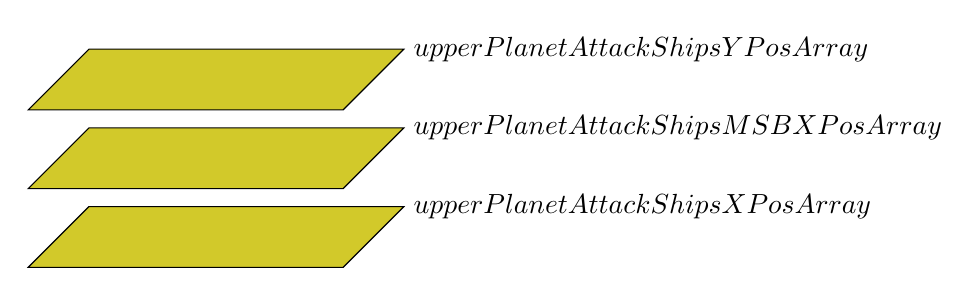
\begin{tikzpicture}
      \draw[fill=yellow!80!black] (0,1,0) -- (4,1,0)--(4,1,2)--(0,1,2)--cycle;
      \node[right] at (4,1,0) {$\icode{upperPlanetAttackShipsXPosArray}$};
      \draw[fill=yellow!80!black] (0,2,0) -- (4,2,0)--(4,2,2)--(0,2,2)--cycle;
      \node[right] at (4,2,0) {$\icode{upperPlanetAttackShipsMSBXPosArray}$};
      \draw[fill=yellow!80!black] (0,3,0) -- (4,3,0)--(4,3,2)--(0,3,2)--cycle;
      \node[right] at (4,3,0) {$\icode{upperPlanetAttackShipsYPosArray}$};
      \end{tikzpicture}
    \end{adjustbox}

  }\caption*{The stack after the code above has run with \icode{upperPlanetAttackShipsXPosArray} at the top.}
\end{figure}

With our position data safely stashed away on the stack we now decide which planet we're on:

\CopyPartialFile{../iridisalpha/src/iridisalpha.asm}{tmp.asm}{2240}{2243}%
\lstinputlisting[]{tmp.asm}

If we're on the upper planet we use \icode{SetXToIndexOfShipThatNeedsReplacing} look in the \icode{activeShipsWaveDataHiPtrArray} for any ships that
need replacing between positions \icode{\$02} and \icode{\$06}. If we don't find one, we return early:

\CopyPartialFile{../iridisalpha/src/iridisalpha.asm}{tmp.asm}{2245}{2249}%
\lstinputlisting[]{tmp.asm}

If we do find one we can now pull (or 'pop') the positional data we stored away in the stack and assign that to the once-dead
ship. First we use the index we retrieved to \icode{X} to get the ship's index (\icode{Y}) into the positional arrays:

\CopyPartialFile{../iridisalpha/src/iridisalpha.asm}{tmp.asm}{2251}{2253}%
\lstinputlisting[]{tmp.asm}

Then we pop the first positional item \icode{upperPlanetAttackShipsYPosArray} from the top of the stack and store in the new
ship's position in the array:

\CopyPartialFile{../iridisalpha/src/iridisalpha.asm}{tmp.asm}{2254}{2255}%
\lstinputlisting[caption="\icode{PLA} remove the top item from the stack and stores it in \icode{A}]{tmp.asm}

The stack now looks like this, popping from the stack has the effect of removing the first item:

\begin{figure}[H]
  {
    \setlength{\tabcolsep}{3.0pt}
    \setlength\cmidrulewidth{\heavyrulewidth} % Make cmidrule = 
    \begin{adjustbox}{width=10cm,center}
      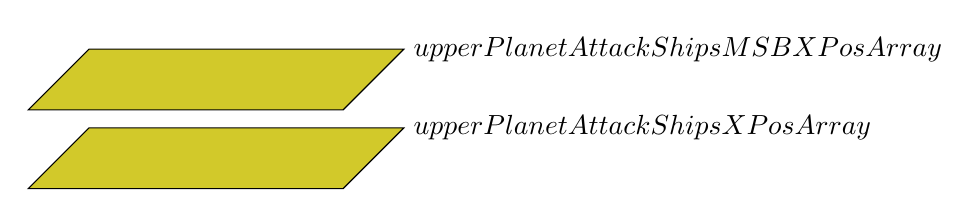
\begin{tikzpicture}
      \draw[fill=yellow!80!black] (0,2,0) -- (4,2,0)--(4,2,2)--(0,2,2)--cycle;
      \node[right] at (4,2,0) {$\icode{upperPlanetAttackShipsXPosArray}$};
      \draw[fill=yellow!80!black] (0,3,0) -- (4,3,0)--(4,3,2)--(0,3,2)--cycle;
      \node[right] at (4,3,0) {$\icode{upperPlanetAttackShipsMSBXPosArray}$};
      \end{tikzpicture}
    \end{adjustbox}

  }
\end{figure}

Then we pop the rest of the items one by one and assign them to the new ship. We ignore the sprite's MXB offset if it is
zero:
\CopyPartialFile{../iridisalpha/src/iridisalpha.asm}{tmp.asm}{2256}{2264}%
\lstinputlisting[caption="\icode{PLA} remove the top item from the stack and stores it in \icode{A}]{tmp.asm}

Now that we have set up the positional data for the new enemy we load all its other features from the data pointed
to by Byte 8-9:

\CopyPartialFile{../iridisalpha/src/iridisalpha.asm}{tmp.asm}{2266}{2269}%
\lstinputlisting[]{tmp.asm}

Let's take a closer look at this routine \icode{UpdateWaveDataPointersForCurrentEnemy}. What it does in this
instance is take the address pointed to by Bytes 8 and 9 and load the data there using the routine
\icode{GetWaveDataForNewShip}. To be used in this way the values in Bytes 8 and 9 are combined and treated
as an address in memory. For example if Byte 8 contains \icode{\$70} and Byte 9 contains \icode{\$13} they
are treated as providing the address \icode{\$1370}. This is the location where the enemy data for
\icode{planet1Level8Data} is kept so that is what is loaded.



\begin{table}[H]
  {
    \setlength{\tabcolsep}{3.0pt}
    \setlength\cmidrulewidth{\heavyrulewidth} % Make cmidrule = 
    \begin{adjustbox}{width=7cm,center}
      \begin{tabular}{rrll}
        \toprule
        Planet &   Level & Byte 7    & Bytes 8-9                   \\
        \midrule
        1 &      11 & \$03       & smallDotWaveData         \\
        1 &      14 & \$03       & planet1Level8Data        \\
        2 &      19 & \$0C       & landGilbyAsEnemy         \\
        3 &       4 & \$04       & gilbyLookingLeft         \\
        3 &       6 & \$04       & planet3Level6Additional  \\
        4 &      19 & \$01       & planet4Level19Additional \\
        5 &       3 & \$01       & planet5Level3Additional  \\
        5 &       5 & \$05       & planet5Level5Additional  \\
        5 &      14 & \$06       & llamaWaveData            \\
        \addlinespace
        \bottomrule
        \multicolumn{4}{@{}l@{}}{Byte 7 : Whether a specific attack behaviour is used.}\\
        \multicolumn{4}{@{}l@{}}{Bytes 8-9 : Lo and Hi Ptr for alternate enemy mode}\\
      \end{tabular}

    \end{adjustbox}

  }\caption{Actual use of Bytes 7, 8, and 9. Note that the value in Byte 7 doesn't matter, as long as it's non-zero.}
\end{table}



\subsection{Enemy Behaviour}


\subsection{Level Movement Data}
